\documentclass[hyperref]{ctexart}
\usepackage[left=2.50cm, right=2.50cm, top=2.50cm, bottom=2.50cm]{geometry} %页边距
\usepackage{helvet}
\usepackage{amsmath, amsfonts, amssymb} % 数学公式、符号
\usepackage[english]{babel}
\usepackage{graphicx}   % 图片
\usepackage{url}        % 超链接
\usepackage{bm}         % 加粗方程字体
\usepackage{multirow}
\usepackage{booktabs}
\usepackage{algorithm}
\usepackage{algorithmic}

\usepackage{amsmath} % 大于等于号有bug
\usepackage{amssymb}

\renewcommand{\algorithmicrequire}{ \textbf{Input:}}       
\renewcommand{\algorithmicensure}{ \textbf{Initialize:}} 
\renewcommand{\algorithmicreturn}{ \textbf{Output:}}     
%算法格式
\usepackage{fancyhdr} %设置页眉、页脚
\pagestyle{fancy}
\lhead{}
\chead{}
\lfoot{}
\cfoot{}
\rfoot{}
\usepackage{hyperref} %bookmarks
\hypersetup{colorlinks, bookmarks, unicode} %unicode
\usepackage{multicol}
\title{\textbf{What affects outcome of attempt in Robotutor?\\ \% correct attempt analysis and prediction}}
\author{\sffamily Yichuan Zhang, \sffamily Nicole Song}
\date{}

\begin{document}
	\maketitle
		\noindent{\bf Abstract: }The Intelligent Tutoring System(ITS) provides tutoring more scientifically. It is helpful when children do not attend school due to the lack of teachers in some developing countries. To achieve this goal better, we can adjust the difficulty of items and the number of practices in RoboTutor by analyzing children's behavior and performance. The percentage of correct attempt prediction is also helpful in the future.\\
		
%		\noindent{\bf Keywords: }Keyword1; Keyword2; Keyword3;...
	\begin{multicols}{2}
	\section{Introduction}
    Intelligent Tutoring System(ITS) is a computer program-based system with models of instructional content for representing knowledge and carrying on interaction with students about what to teach and the teaching strategies. To better understand how students interact with coursework, Knowledge Tracing(TC) and data analysis can provide insights to infer which subjects and problems children's mastery.
    
    
    Robotutor is an open-source application that provides individual help and feedback to children aged 7-10 who are affected by a lack of teachers. Robotutor uses a variety of items such as counting numbers and story reading to teach children. In this paper, to specify more correctly about what to teach and how to teach, analyzing children's performance and their study behavior is crucial to adjust the proper estimation of their level and proceed accordingly. Two parts will be analyzed after the Robotutor collects data from each tablet. The data analysis part includes: What is the hardest part and what is the easiest? Do lettercases differences affect children's performance? Do stimulus modalities differences affect children's performance? Then, we applied data to logistic regression and random forest model to predict the percentage of correct attempts for each child.
    
    
    The data set we used was the transaction table recorded by the Robotutor when it was testing in Africa.

	\subsection{Matrix and Tutor Name Introduction with Interface Snapshots}
	To let children who lack educational resources learn reading, writing, and simple arithmetic skills, Robotutor provides a variety of items. We can divide them into three matrices according to what we want to teach: literacy, math, and story. Specifically,
\begin{itemize}
\item \textbf{}
    Literacy focuses on language learning for beginners. It mainly introduces the user to recognize letters and syllables.
\item \textbf{}
    Math mainly trains children to recognize Arabic numerals and master some simple addition calculations. Also, it uses animation and pictures to help children understand the size of numbers.
\item \textbf{}
    Story is designed to enhance the ability of users to listen and read. It provides children with long texts and helps them read and understand.
\end{itemize}
    
    
    Robotutor uses a variety of items to help children learn language and mathematics. We use tutor names to describe various items. According to the teaching needs, different kinds of matrices can use the same type of item, as we can use Akira in both "literacy" and "math." In other words, an item is a question pattern designed to help children to learn. As shown below, there are some joint items.

	\subsubsection{Bubble Pop}
    Bubble pop, also known as Bpop, is one of the most common items. It has several variants and is frequently-used in literacy and math items.


    In bubble pop, the user needs to select the bubble with the correct answer from all the bubbles. Bubble pop is divided into "show" and "no show", as shown in the figure 1 and figure 2, the Bpop of the "show" type will give children a direct visual prompt at the bottom of the screen.
    
    \begin{figure}[H]
    \small
    \centering
    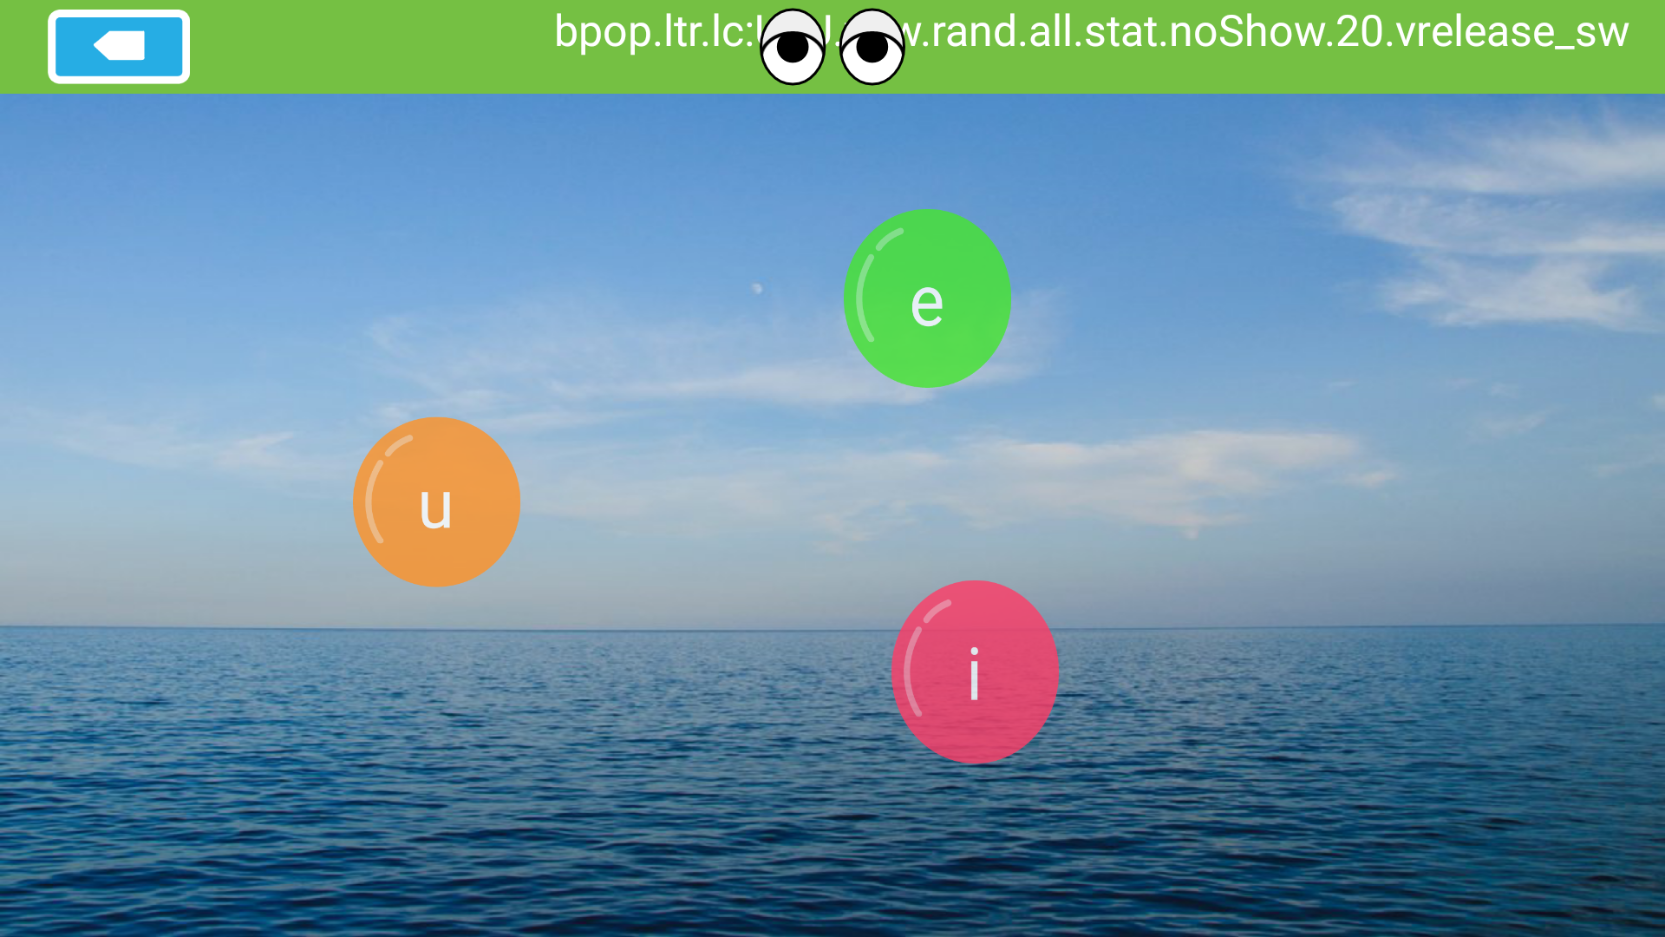
\includegraphics[width=8cm]{1.png}
    \caption{Bubble Pop "no show"} \label{fig:aa}
    \end{figure}
    
    \begin{figure}[H]
    \small
    \centering
    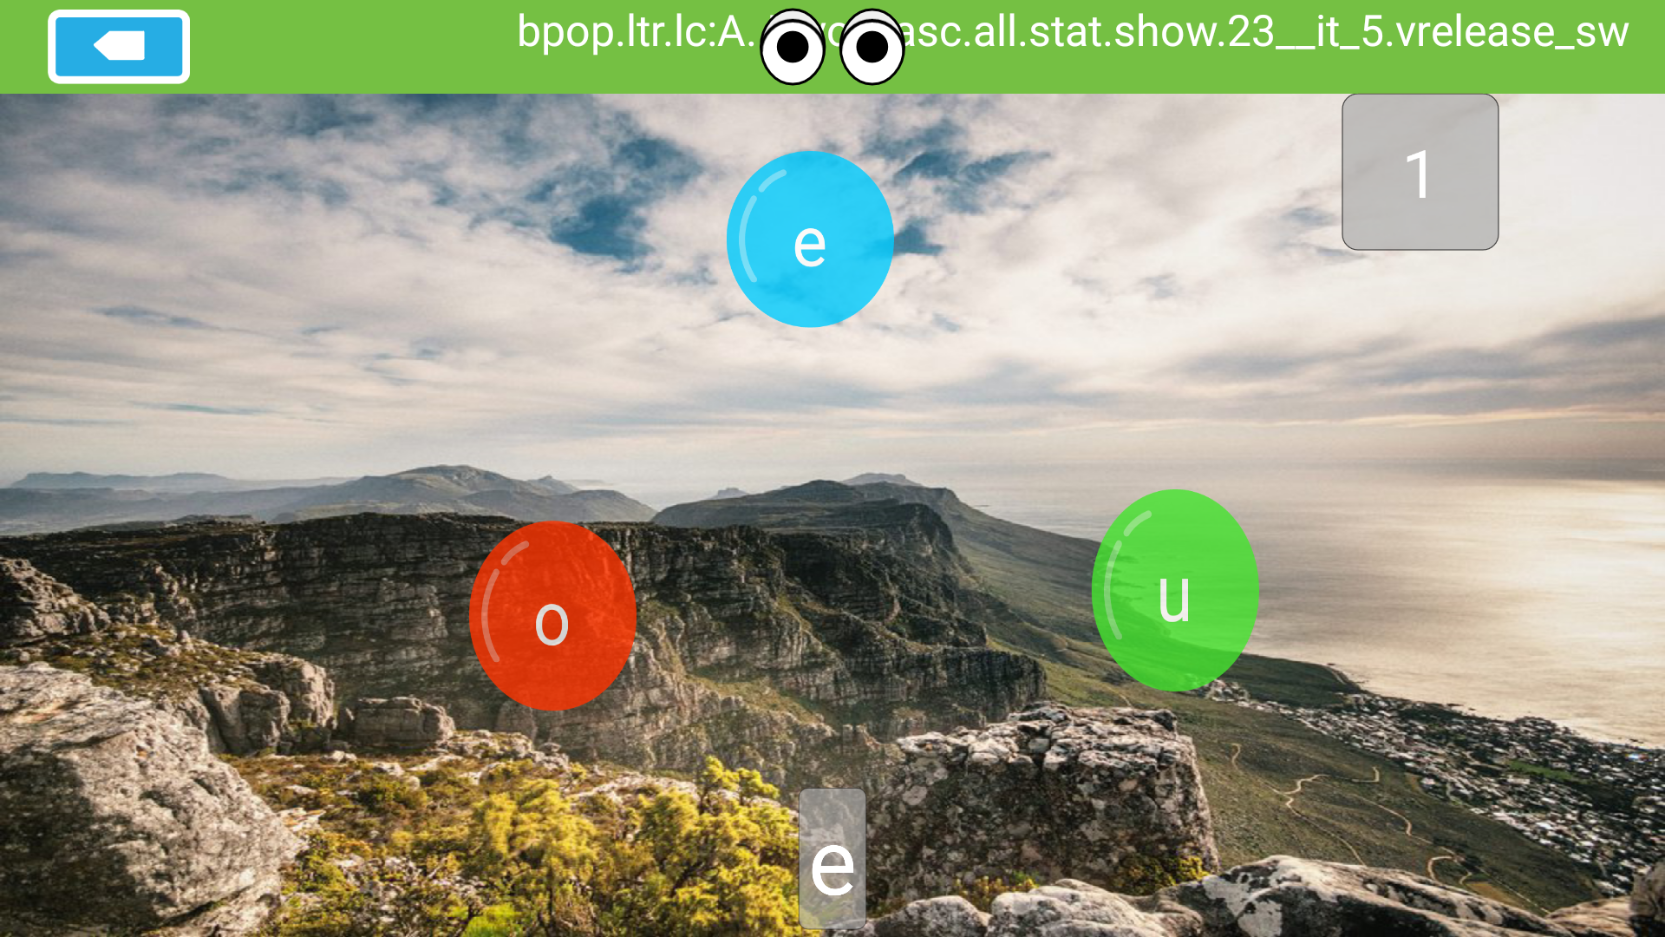
\includegraphics[width=8cm]{2.png}
    \caption{Bubble Pop "show"} \label{fig:aa}
    \end{figure}
    
    Also, there is a variant of bubble pop called "rise." In this kind of bubble pop, bubbles are not fixed but rise from the bottom of the screen until they exceed the top of the screen. Children need to select bubbles in time before they leave the screen. Bubbles will continue to be generated from the bottom before students find the right bubble.
    \begin{figure}[H]
    \small
    \centering
    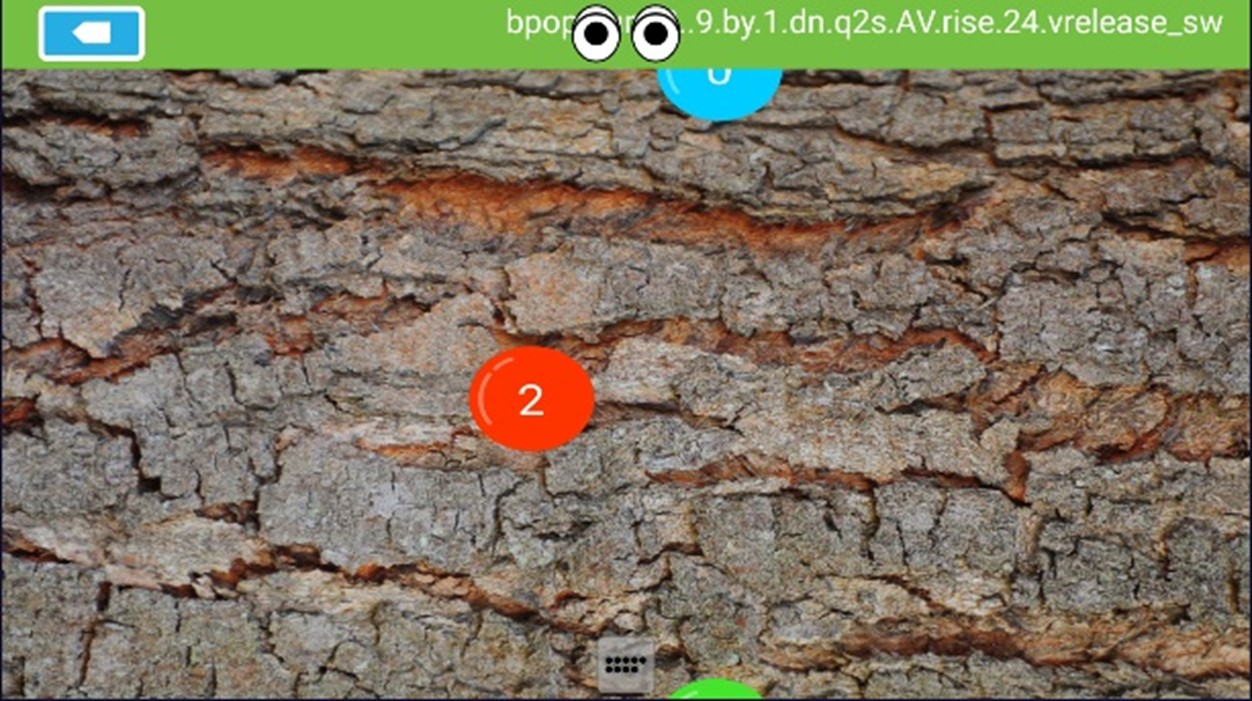
\includegraphics[width=8cm]{3.jpg}
    \caption{Bubble Pop "rise"} \label{fig:aa}
    \end{figure}
    
    \subsubsection{Akira}
    Akira is a racing car game. Children need to control the car to cross the terminal. As shown in the figure 4, only one of the three roads the red car faces is the correct answer. Children need to click on the proper route to let the car change road and drive through it. However, unlike bubble pop, Akira has a time limit. Children must choose before they run into obstacles. Akira also has two types as "show" and "no show." Like bubble pop, Akira with "show" has visual prompts.
    \begin{figure}[H]
    \small
    \centering
    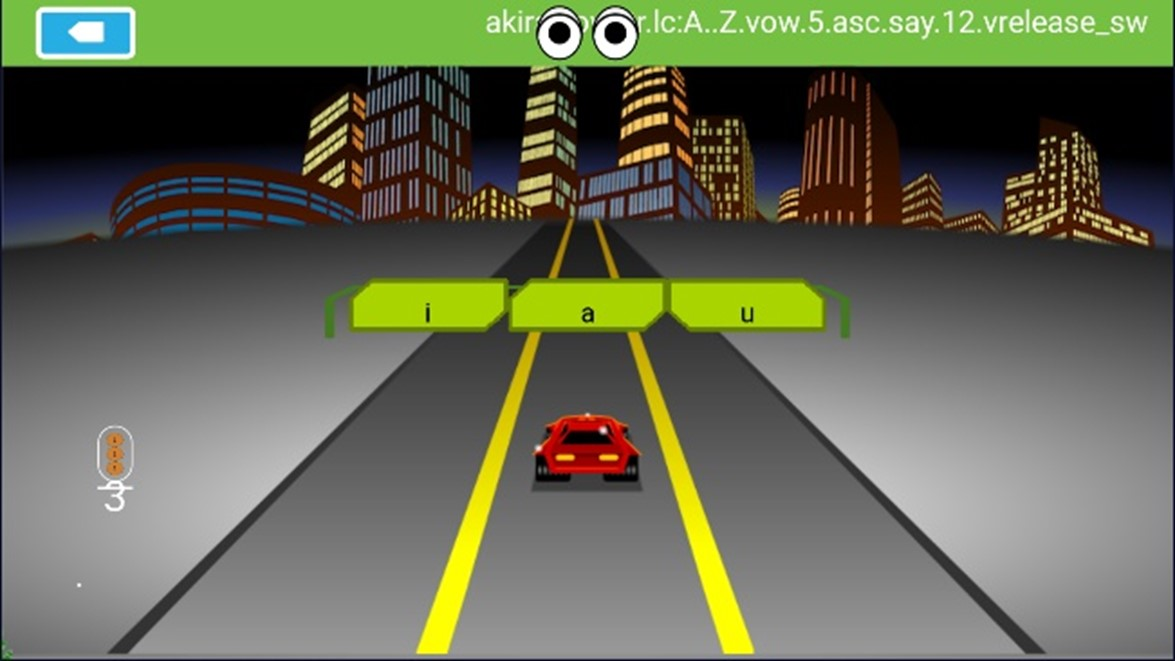
\includegraphics[width=8cm]{4.jpg}
    \caption{Akira} \label{fig:aa}
    \end{figure}
    
    \subsubsection{Word Copy}
    In word copy, children need to write numbers in the writing area of the screen as required. The Robotutor will automatically recognize the input number and judge whether it is correct or not. There are many variations of word copy. One of the main differences is how the Robotutor displays the number it needs, which can be pictures or audio.
    \begin{figure}[H]
    \small
    \centering
    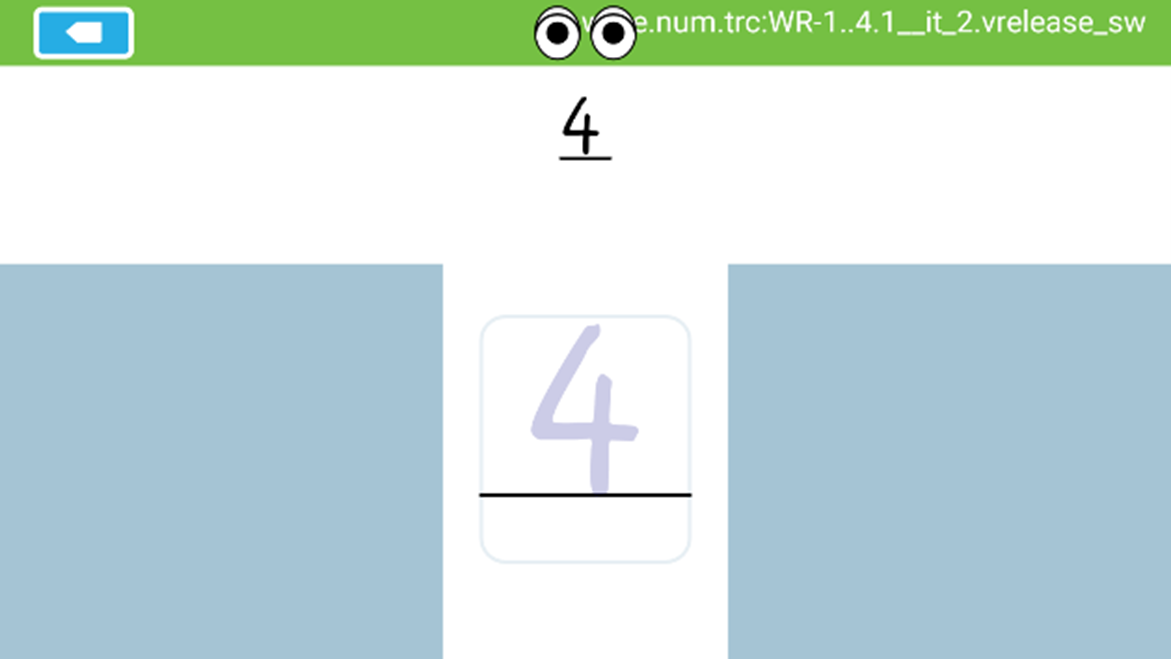
\includegraphics[width=8cm]{5.png}
    \caption{Word Copy} \label{fig:aa}
    \end{figure}
    
    \subsubsection{Story Reading}
    Robotutor will play audio to the child. The audio can be a story or a song. Most story readings don't need any answers from users, so we call them passive questions
    \subsubsection{Countingx}
    In countingx, the Robotutor will provide a number to the child. The child needs to click on the screen. Each click adds an object. When the number of clicks reaches, the animation will be played. All the objects will move into a box of 10 squares to help the child understand the size of the number visually.


	\section{Analyze Factors that Affect \% Correct Attempt}
	\subsection{Effect of Attempt Number on \% Correct Attempt}
	Figure 6 shows the relationship between attempt number and \% correct attempt.
	
	\begin{figure}[H]
    \small
    \centering
    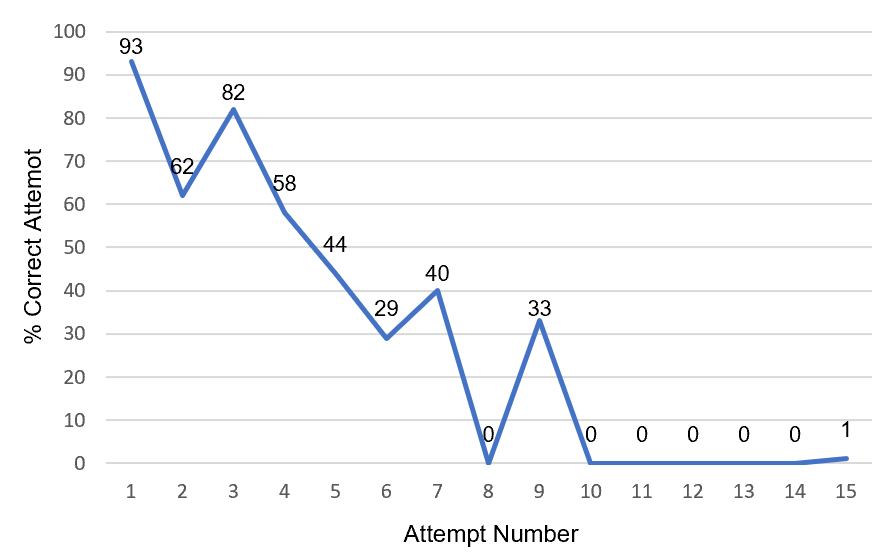
\includegraphics[width=8cm]{attemptnum.png}
    \caption{\% Correct Attempt by Attempt Number} \label{fig:aa}
    \end{figure}
	

    When the attempt number is greater than 6, the data we collected is very insufficient. This is normal since most of the items have 3-strike restrictions, which means these items' attempt numbers will not exceed 3. In addition, Datashop treats an item as correct only if it is right on the first attempt without help requests. As shown in the figure, children's \% correct attempt is the highest at the first attempt, decreasing the subsequent shots. We believe that this phenomenon could be explained by a sample skew, as the fast correct answers drop out of the pool. The remaining data is from children wrong on the first attempt, and these children are random guessers who will make more attempts before succeeding. The phenomenon of trying many times appears in few students. Considering that after the first attempt, children already know a wrong answer, and some may take multiple shots as a learning skill, which leads to the later attempts to no longer represent the user's actual level. What is more, we calculated \% correct attempt when attempt number =1 and \textgreater 1, and found that the former is significantly higher, 93\% \textgreater 66\%.

    
    
    According to the above, in the later study of \% correct attempt, we only select those attempts with attempt number equal to 1.


	\subsection{Relationship Between Tutor Name and \% Correct Attempt}
	The percentage of correct attempts for literacy, story and math are 97\%, 99\% and 78\% respectively. Considering that different items need different completion methods, in order to reveal the relationship between activity and \% correct attempt more accurately, we analyze by the type of item, also known as tutor name.
	
		\begin{figure}[H]
    \small
    \centering
    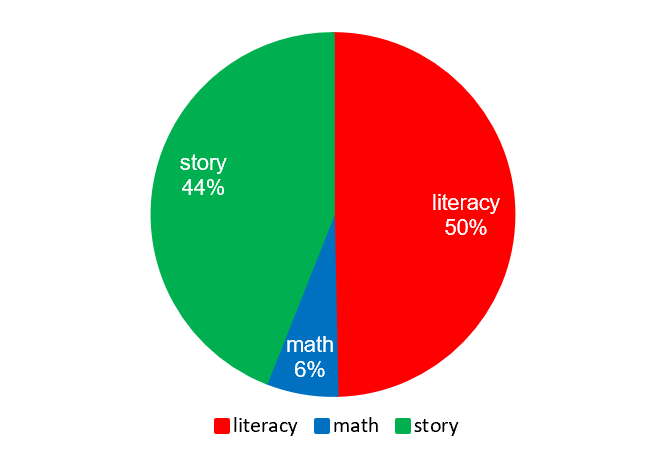
\includegraphics[width=8cm]{pie.png}
    \caption{The Proportion of 3 Matrices in All Items
} \label{fig:aa}
    \end{figure}
    
	\begin{figure}[H]
    \small
    \centering
    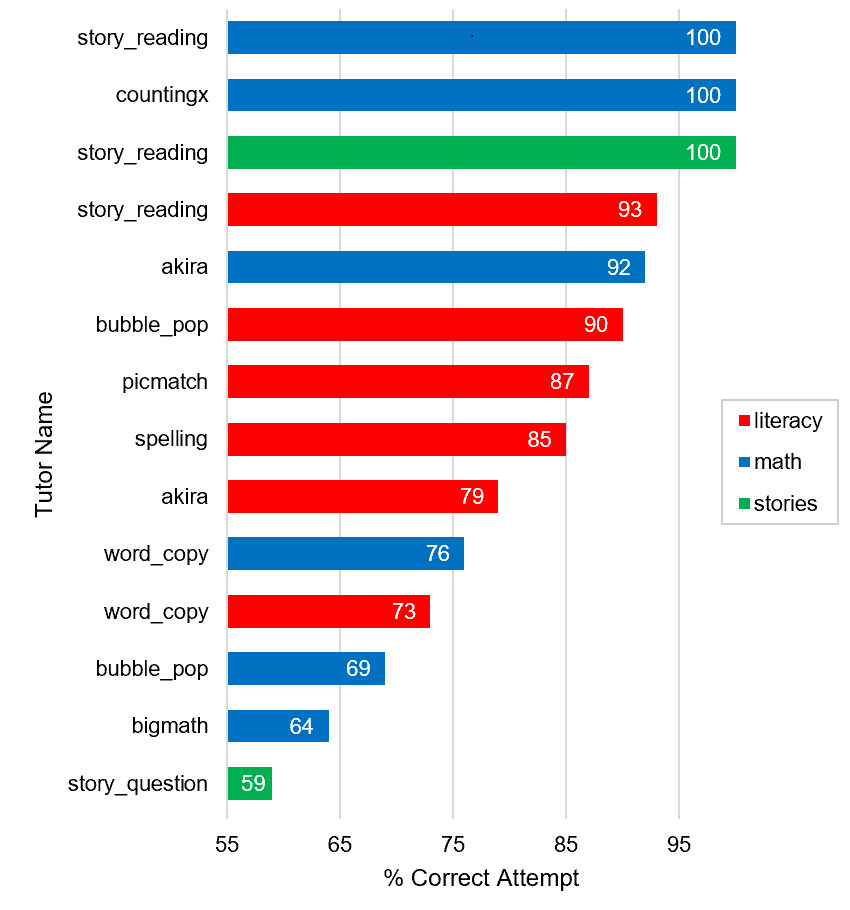
\includegraphics[width=8cm]{tutorname.png}
    \caption{\% Correct Attempt by Tutor Name
} \label{fig:aa}
    \end{figure}
	
	As shown in the figure 8, we can see the story reading and countingx have the highest \% correct attempts. It is because these two kinds of questions are almost passive questions. Children don't need to answer any questions. So the Robotutor will take it as correct.
	
	
    From the perspective of \% correct attempt, story\_questions, bigmath, and bubble\_pop(math) are three items with the lowest correct rate, which are 59\%, 64\%, and 69\% separately.
    
    
    If we remove the passive questions, and group all the items by their matrix, then literacy items have higher \% correct attempt than math ones.
    
    
    From all items, the children have the fewest activities in math, and the \% correct attempt of math is lower than literacy and story, so compared with the other two subjects, math items are relatively hard for children.


\subsection{The Influence of Letter Case Change on \% Correct Attempt}
There are uppercase and lowercase differences for different tutor name items. For example, Akira, BPOP, write, story echo, and story hear. Uppercase \% correct attempts are higher in Akira and BPOP and write.


There is no apparent difference between the \% correct attempt of upper case letters and lowercase letters for the story. Lower case letters may be more confusable than uppercase letters -- for kids but also handwriting recognizers.

\begin{table}[H]
  \begin{tabular}{lll}
    \noalign{\global\arrayrulewidth1pt}\hline\noalign{\global\arrayrulewidth0.4pt}
    &\quad lowercase\quad\quad& uppercase\quad\quad&
    \hline
    akira.all.ltr&  \quad \quad 77\%& \quad 83\%& 
    bpop.ltr&       \quad \quad 87\%& \quad 95\%&
    story.echo&     \quad \quad 98\%& \quad 99\%&
    story.parrot&   \quad \quad 98\%& \quad 97\%&
    write.ltr&      \quad \quad 72\%& \quad 85\%&
    \noalign{\global\arrayrulewidth1pt}\hline\noalign{\global\arrayrulewidth0.4pt}
  \end{tabular}
  \caption{\% Correct Attempt by Letter Case and Tutor Name}
\end{table}

\subsection{Stimulus Modality}
We find all items with "show" and "noshow" stimulus modalities in the dataset and calculate their \% correct attempt. As shown in the following table, the \% correct attempt is significantly different under different stimulus modalities, and the \% correct attempt of items with show type is higher.
\begin{table}[H]
  \begin{tabular}{lll}
    \noalign{\global\arrayrulewidth1pt}\hline\noalign{\global\arrayrulewidth0.4pt}
    &\quad\quad noshow\quad\quad&\quad\quad show\quad\quad\quad&
    \hline
    bpop.ltr.lc&       \quad\quad \quad 82\%& \quad\quad 89\%&
    bpop.ltr.uc&       \quad\quad \quad 93\%& \quad\quad 95\%&
    bpop.wrd&          \quad\quad \quad 81\%& \quad\quad 88\%&
    \noalign{\global\arrayrulewidth1pt}\hline\noalign{\global\arrayrulewidth0.4pt}
  \end{tabular}
  \caption{\% Correct Attempt by Stimulus Modality and Tutor Name}
\end{table}

\subsection{Akira vs. Bpop}
We noticed that some problems could be designed for both Akira problems and bubble pop problems. E.g., choose 'i' from 'a', 'i', and 'o'. We explored the dataset to see if the type of problem has an impact on \% correct
 
 
The content of the item is the same when Akira and BPOP can replace each other, e.g., choose the correct letter. Since Akira has three options for each attempt, The corresponding bubble pop we choose should also have three bubbles for each item; that is to say, we should exclude all bubble pop of rising type. The Akira and Bubble pop that can replace each other should have the same kind of stimulus modality; in our dataset, this is "noshow."
 
Then we found some replaceable literacy Bpop and literacy Akira in the dataset.
\begin{table}[H]
  \begin{tabular}{lll}
    \noalign{\global\arrayrulewidth1pt}\hline\noalign{\global\arrayrulewidth0.4pt}
    &\quad\quad Bpop(noshow)\quad\quad&\quad\quad Akira\quad\quad\quad&
    \hline
    *.ltr.lc&       \quad\quad \quad 82\%& \quad\quad 77\%&
    *.ltr.uc&       \quad\quad \quad 93\%& \quad\quad 82\%&
    \noalign{\global\arrayrulewidth1pt}\hline\noalign{\global\arrayrulewidth0.4pt}
  \end{tabular}
  \caption{\% Correct Attempt by Akira and Bubble Pop}
\end{table}

If a Bpop has a replaceable Akira, then the \% correct attempt of this Bpop is higher than the corresponding Akira. There are two main reasons for the difference in accuracy: first, Akira has time pressure. Second, Akira's question is moving, unlike fixed position bubbles, which are relatively easier to identify quickly.
	

\section{Models to Predict \% Correct Attempt}
\subsection{Preprocessing}
We delete all attempts of passive problems. Since the \% correct attempt of these problems are always 100\%, We deleted rows with a null value. Crashes mainly cause these.

    \begin{figure}[H]
    \small
    \centering
    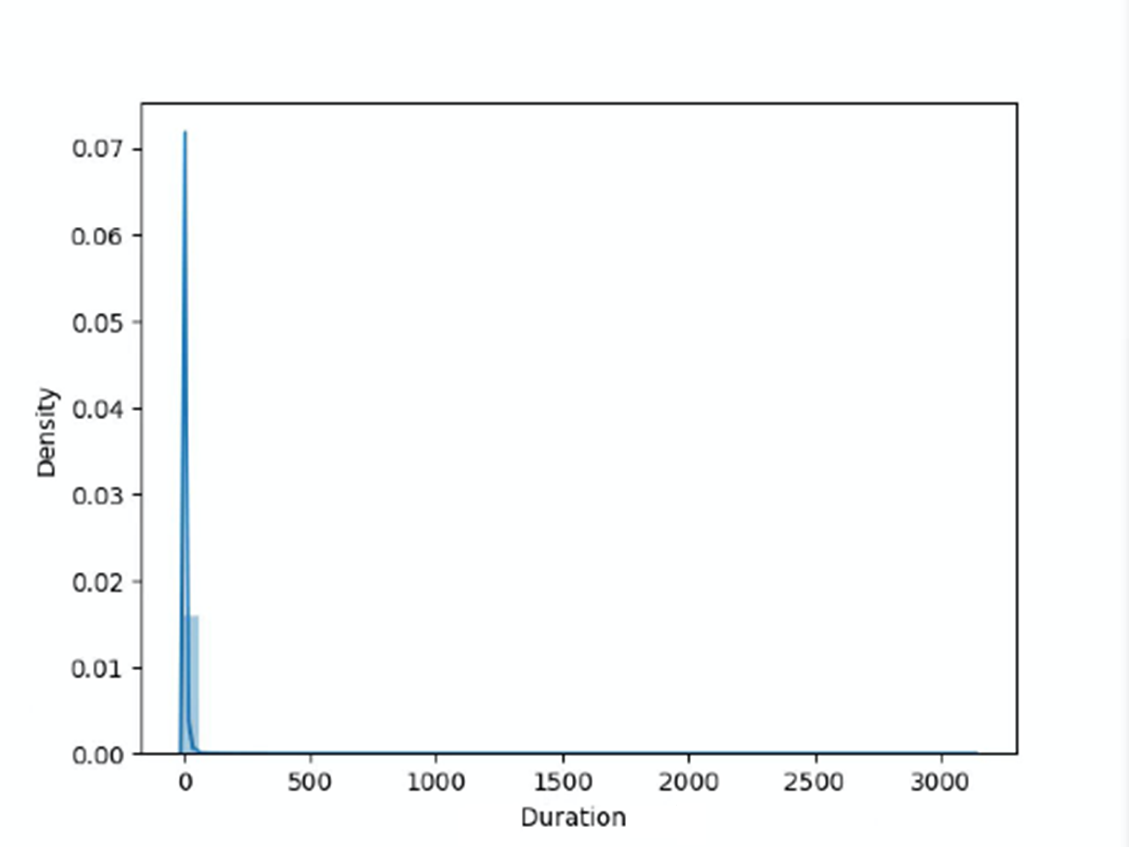
\includegraphics[width=8cm]{duration1.png}
    \caption{Before Preprocessing} \label{fig:aa}
    \end{figure}
    
    
In processing of duration, we find that there is some too large data, which may be caused by long thinking time, leaving halfway, or program crash. As a result, the distribution of duration does not satisfy the normal distribution. We take a logarithm and divide it by log (max) to make the duration close to the normal distribution and make the maximum minus the minimum less than 1. Then we delete all durations that are greater than the average plus three times the standard deviation. These excessive durations account for 0.7\% of the total data.

    \begin{figure}[H]
    \small
    \centering
    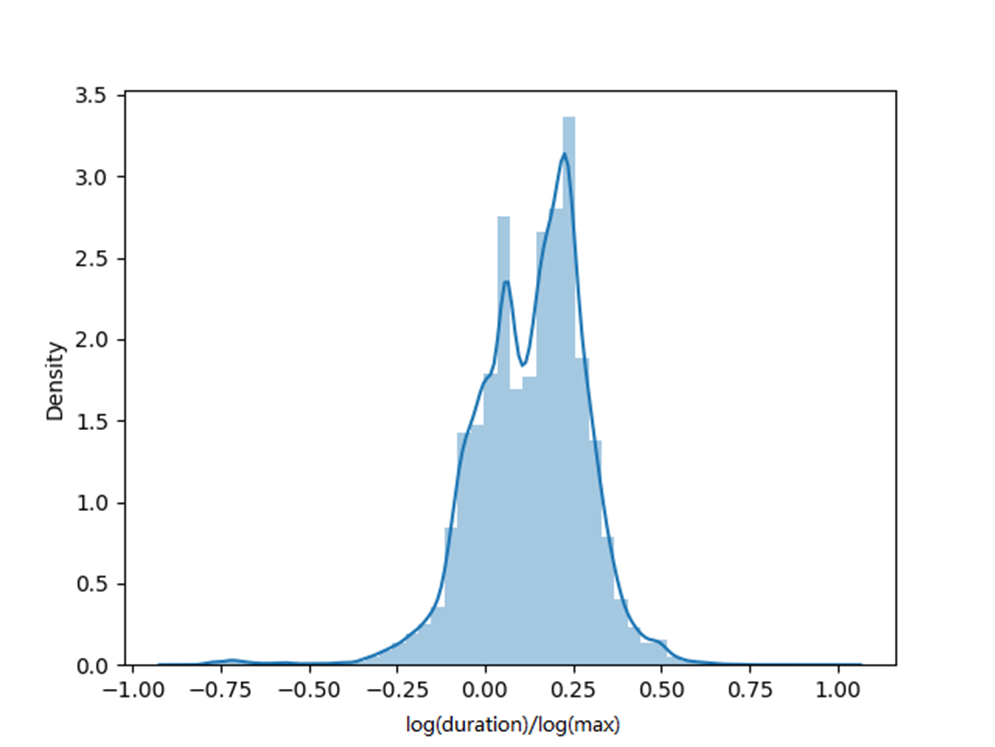
\includegraphics[width=8cm]{duration2.png}
    \caption{After Preprocessing} \label{fig:aa}
    \end{figure}

We use one-hot encoding to transform all discrete features into continuous features. We calculate the correlation matrix for better feature selection and remove all the columns whose correlation is close to one.


To predict the outcome of an attempt, we regard it as a classification problem. The result is divided into two types: success and failure. Therefore, it is suitable for a logistic regression model to predict the outcome.


Then, we trained a random forest model to predict the outcome.

\subsection{Leave-1-Student-Out Validation}
Since the dataset we used is relatively small and contains less than ten anon student IDs, we used leave-1-student-out cross-validation to predict performance on unseen students.


We use grid search to find a set of optimal parameters of the model.
\subsection{Model Evaluation}
    \begin{figure}[H]
    \small
    \centering
    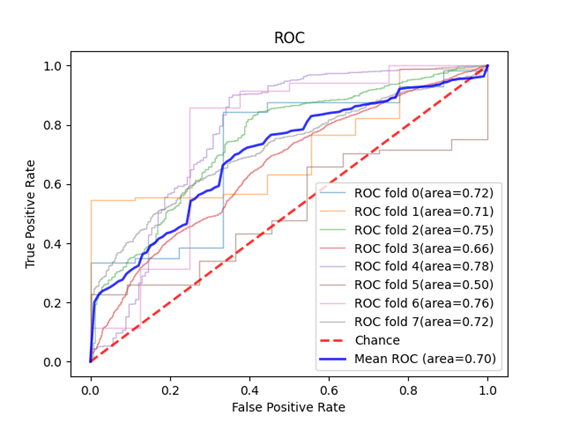
\includegraphics[width=8cm]{LRROC.png}
    \caption{ROC of Logistic Regression} \label{fig:aa}
    \end{figure}

    \begin{figure}[H]
    \small
    \centering
    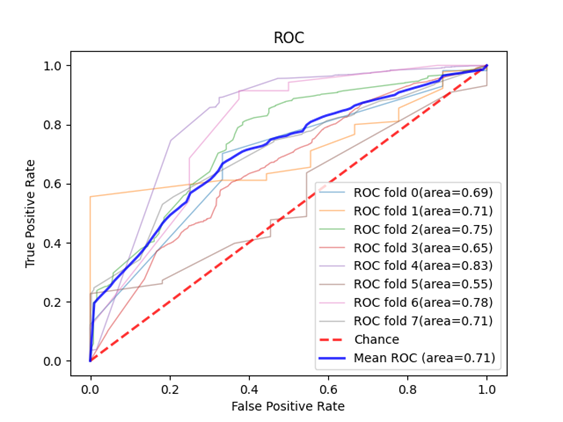
\includegraphics[width=8cm]{RFROC.png}
    \caption{ROC of Random Forest} \label{fig:aa}
    \end{figure}
As shown in the figure 11 and figure 12, our two models are verified by leave-1-student-out method, and the average AUC of ROC curve is 0.70 and 0.71 respectively.

\begin{table}[H]
  \begin{tabular}{lll}
    \noalign{\global\arrayrulewidth1pt}\hline\noalign{\global\arrayrulewidth0.4pt}
    &\quad\quad LR\quad\quad& \quad RF&
    \hline
    Mean Accuracy\\(leave-1-student-out)&  \quad \quad 77.13\%& \quad 77.24\%& 
    \hline
    Mean Accuracy\\(10-fold)&       \quad \quad 84.42\%& \quad 84.87\%&
    \hline
    AIC\\(Akaike information criterion)&       \quad \quad 19725& \quad 19718&
    \hline
    BIC\\(Bayesian InformationCriterion)&       \quad \quad 19798& \quad 19791&
    \hline
    Sensitivity&       \quad \quad 0.99& \quad 1.00&
    \hline
    Precision&       \quad \quad 0.88& \quad 0.85&
    \hline
    \noalign{\global\arrayrulewidth1pt}\hline\noalign{\global\arrayrulewidth0.4pt}
  \end{tabular}
  \caption{Model Evaluation of Logistic Regression(LR) and Random Forrest(RF)}
\end{table}
	
\section{Conclusion}
According to our research, we think story questions are the most challenging item to answer correctly, while the passive questions are the easiest. What is more, judging from the number of completed items, the children have the lowest interest in math, and the \% correct attempt of math is more melancholy than literacy and story, so we believe that math is a bit too difficult. We suggest that Robotutor add a function to balance the frequency of users using different types of items to achieve a more comprehensive teaching goal.


We also found that lowercase letters may be more confusable than uppercase letters for kids to recognize. Therefore, we suggest providing more training for children to recognize lowercase letters in the future, such as increasing the number of items in lowercase.


We found that stimulus modalities affect users' performance. Giving children a visual cue can significantly increase \% correct attempt.


We compare children's performance of the same problem on Akira and bubble pop and found that Akira is more complex and difficult than a replaceable bubble pop. There are two reasons. First, Akira has time pressure. Second, Akira's question is moving, unlike fixed position bubbles, which are relatively easier to identify quickly.







%	\begin{thebibliography}{100}%此处数字为最多可添加的参考文献数量
%		\bibitem{article1}This is reference.%title author journal 
% data pages
%		\bibitem{book1}This is reference.%title author publish date
%	\end{thebibliography}

\end{multicols}
\end{document}
